\documentclass{article}
\usepackage[utf8]{inputenc}
\usepackage[greek,english]{babel}
\usepackage{alphabeta}
\usepackage{fancyhdr}
\usepackage{listings}
\usepackage{mathtools}
\usepackage{xcolor}
\usepackage{graphicx}
\usepackage{float}
\usepackage[backend=biber]{biblatex}

\title{Σήματα και Συστήματα - Τελική Εργασία}
\author{Χρήστος Μαργιώλης - 19390133}
\date{Ιούνιος 2021}

\begin{document}

\begin{titlepage}
        \maketitle
        \begin{figure}[t!]
        \begin{center}
        
\includegraphics[scale=0.3]{./res/uniwalogo.png} \\
        \Large
        \textbf{Πανεπιστήμιο Δυτικής Αττικής} \\
        \large
        Τμήμα Μηχανικών Πληροφορικής και Ηλεκτρονικών Υπολογιστών
        \end{center}
        \end{figure}
\end{titlepage}

\renewcommand{\contentsname}{Περιεχόμενα}
\tableofcontents

\section{'Ασκηση 1}

\begin{itemize}
	\item Να γραφτεί ο κώδικας για τον υπολογισμό της συνάρτησης
	\[
		x(n) = 
		\left\{
			\begin{array}{lll}
			0 & if & n < 2 \\
			2n-4 & if & 2 \leq n < 4 \\
			4-n & if & 4 \leq n
		\end{array}
		\right.
	\]

\end{itemize}

\begin{lstlisting}[language=octave]
	step = 0.001;
	n1 = -8:step:2;
	x1 = zeros(size(n1));
	n2 = 2:step:4-step;
	x2 = 2*n2-4;
	n3 = 4:step:8;
	x3 = 4-n3;
	n = [n1 n2 n3];
	x = [x1 x2 x3];
	plot(n, x);
\end{lstlisting}

\begin{figure}[H]
	\centering
	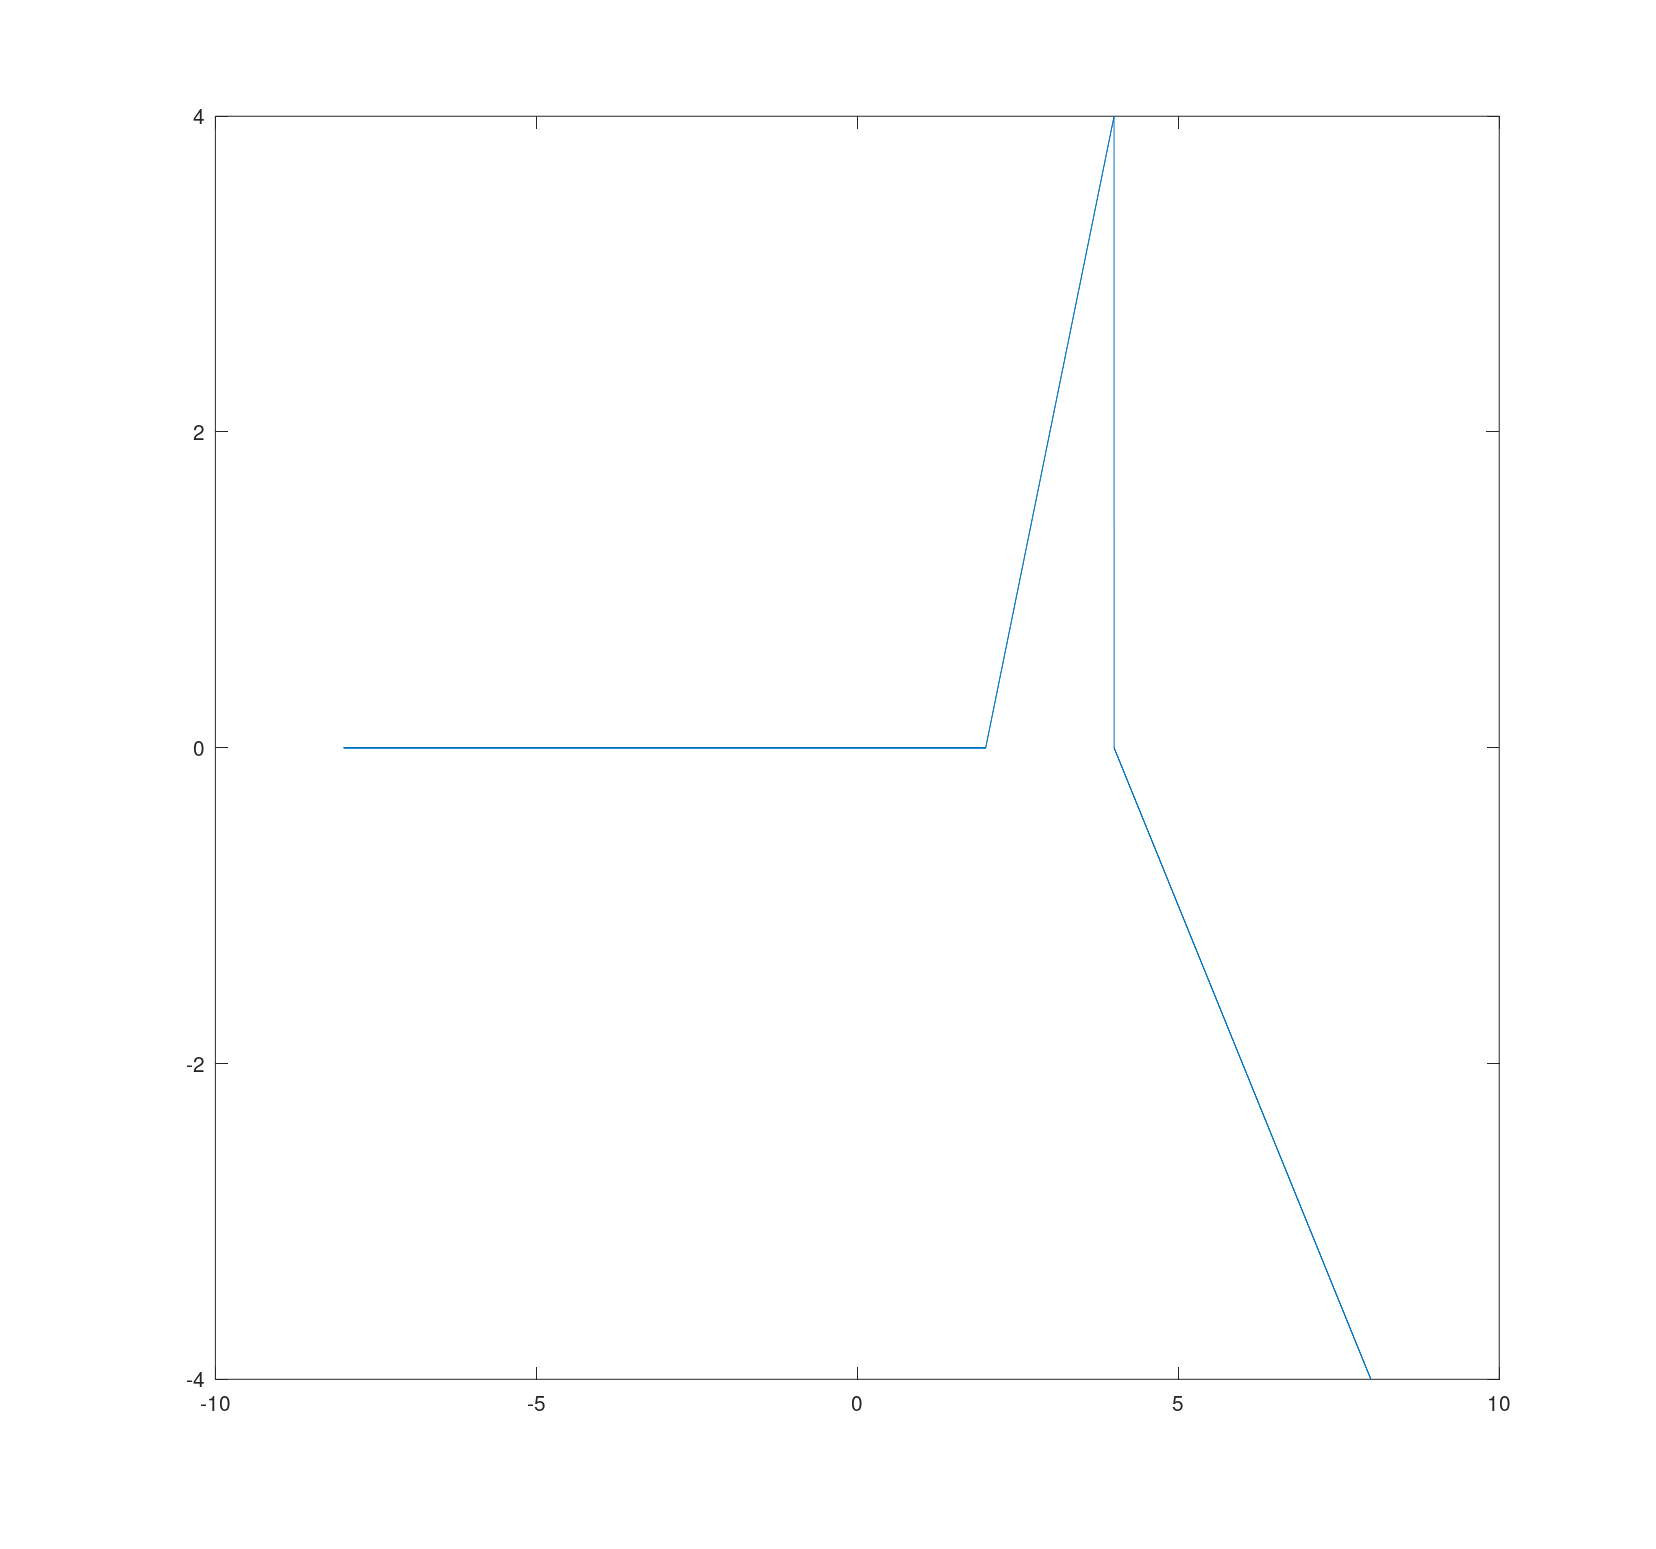
\includegraphics[width=\linewidth]{res/fig1.png}
\end{figure}

\section{'Ασκηση 2}

\begin{itemize}
	\item Να σχεδιαστεί το παρακάτω αναλογικό σήμα:
	\[
		x(t) = 
		\left\{
			\begin{array}{ll}
			0 & t \leq -1 \\
			\cos(\pi t/2) & -1 < t \leq 0 \\
			e^{-t} & 0 < t \leq 1 \\
			0 & 1 < t
		\end{array}
		\right.
	\]
\end{itemize}

Θα ακολουθήσουμε παρόμοια λογική με την άσκηση 1, δηλαδή, θα
υπολογίσουμε το σήμα για κάθε ένα από διανύσματα χρόνου, θα ενώσουμε
όλα τα αποτέλεσματα και θα τα σχεδιάσουμε.

\begin{lstlisting}[language=octave]
	step = 0.001;
	t1 = -3:step:-1;
	x1 = zeros(size(t1));
	t2 = -1+step:step:0;
	x2 = cos(pi * t2 / 2);
	t3 = 0+step:step:1;
	x3 = exp(-t3);
	t4 = 1+step:step:3;
	x4 = zeros(size(t4));
	t = [t1 t2 t3 t4];
	x = [x1 x2 x3 x4];
	plot(t, x);
\end{lstlisting}

\begin{figure}[H]
	\centering
	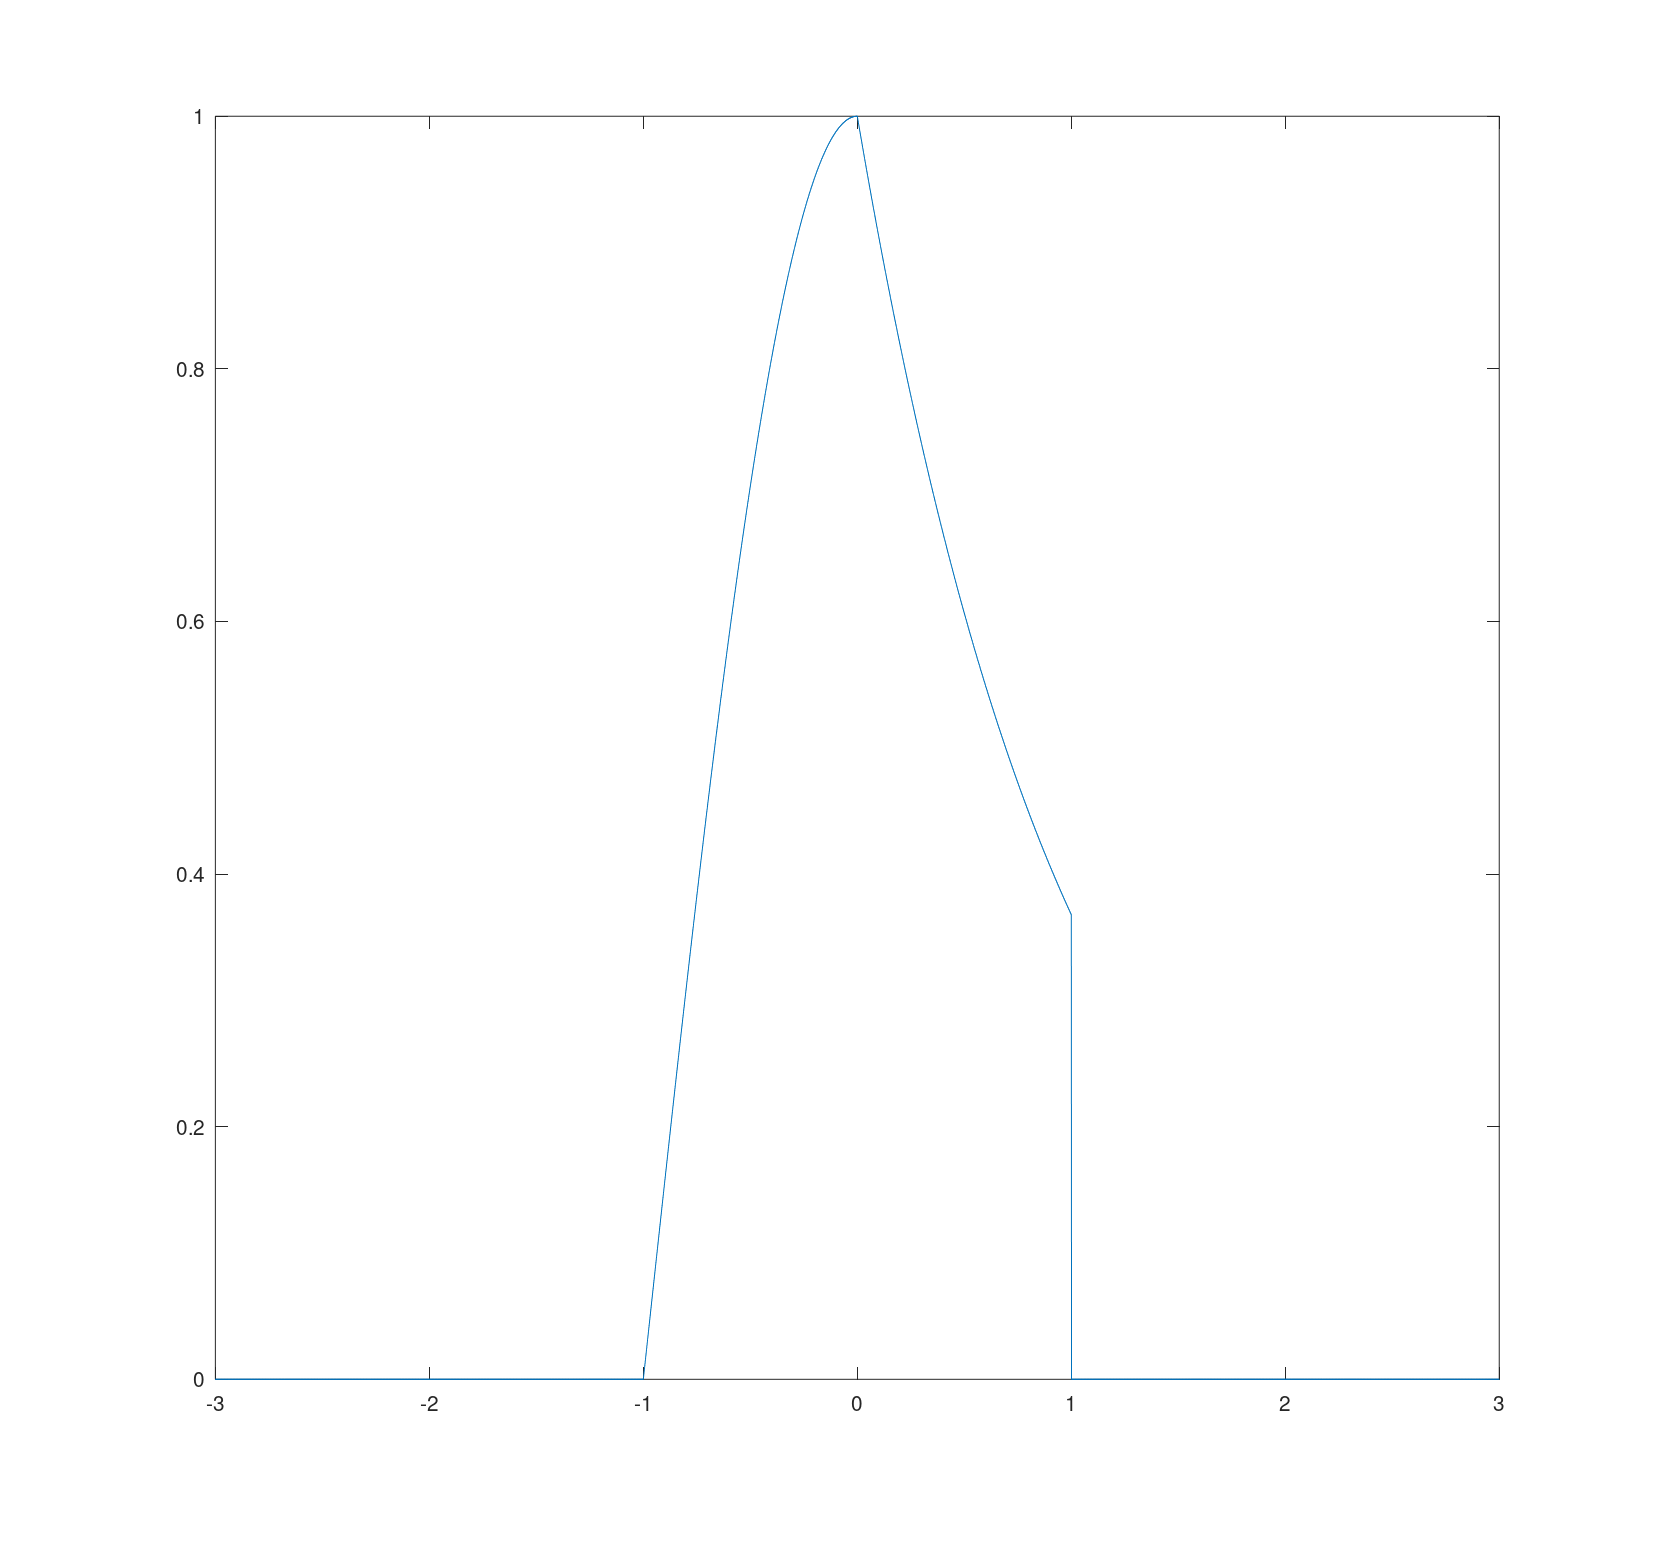
\includegraphics[width=\linewidth]{res/fig2.png}
\end{figure}

\section{'Ασκηση 3}

\begin{itemize}
	\item Να γραφτεί κώδικας για τον υπολογισμό της συνέλιξης των
		συναρτήσεων συνεχούς χρόνου $h(t)$ και $x(t)$.
		\[h(t) = [2te^{-t} + e^{-2t} - e^{-3t}] \cdot u(t)\]
		\[x(t) = [1 - e^{-1.5t}] \cdot u(t)\]
\end{itemize}

Για τον υπολογισμό της συνέλιξης θα χρησιμοποιηθεί η συνάρτηση 
\lstinline{conv()}.

\begin{lstlisting}[language=octave]
	t = 0:0.01:10;
	dt = t(2);
	h = 2*t.*exp(-t)+exp(-2*t)-exp(-3*t);
	x = 1-exp(-1.5*t);
	y = conv(x,h)*dt;
	plot([0:dt:20], y);
\end{lstlisting}

\begin{figure}[H]
	\centering
	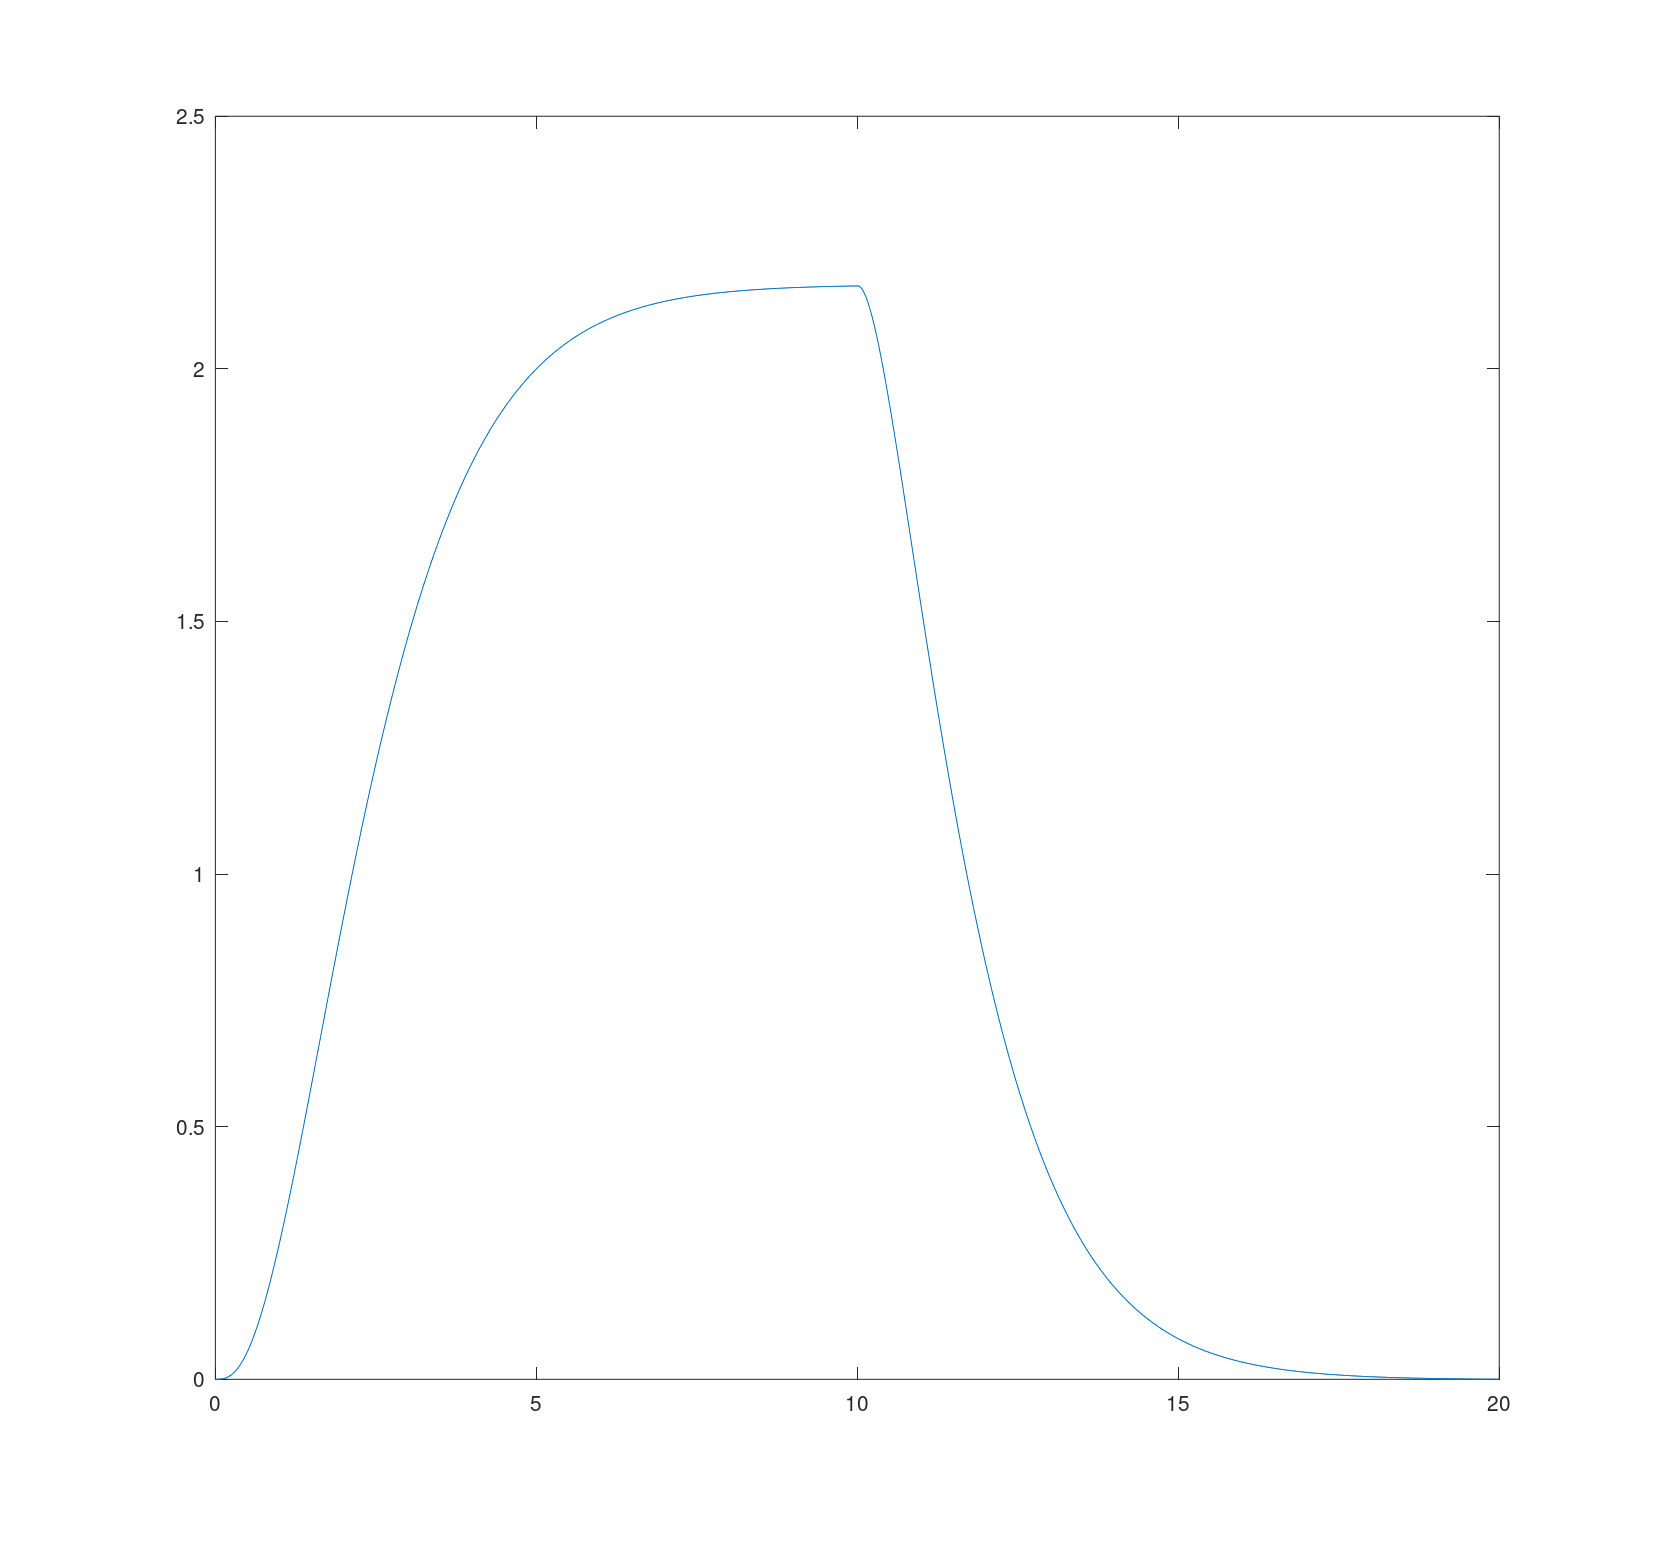
\includegraphics[width=\linewidth]{res/fig3.png}
\end{figure}

\section{'Ασκηση 4}

Δεν έγινε.

\section{'Ασκηση 5}

\begin{itemize}
	\item Να βρεθεί το ανάπτυγμα εκθετικής σειράς Fourier του
		τρένου παλμών που εικονίζεται στο σχήμα ($T = 1\sec$
		η περίοδος) και το σήμα σε διάρκεια μίας περιόδου
		περιγράφεται από τη σχέση:
		\[
			x(t) = 
			\left\{
				\begin{array}{ll}
				2 & 0 \leq t \leq 1/4 \\
				0 & 1/4 < t < 3/4 \\
				2 & 3/4 \leq t \leq 1
			\end{array}
			\right.
		\]
		Να σχεδιαστούν οι προσεγγίσεις για 41, 21, 5 όρους του
		περιοδικού σήματος και να βρεθούν τα αντίστοιχα ποσοστά
		προσέγγισης.
\end{itemize}

\begin{lstlisting}[language=octave]
	step = 0.001;
	t1 = 0:step:1/4;
	x1 = 2.*ones(size(t1));
	t2 = 1/4+step:step:3/4-step;
	x2 = zeros(size(t2));
	t3 = 3/4+step:step:1;
	x3 = 2.*ones(size(t3));
	t = [t1 t2 t3];
	x = [x1 x2 x3];
	plot(t, x);

	syms t;
	x = 1+(heaviside(t)-heaviside(t-(1/4))) ...
		- (heaviside(t-(1/4))-heaviside(t-(3/4))) ...
		- (-heaviside(t-(3/4))+heaviside(t-1));
	ezplot(t, [0 1]);

\end{lstlisting}

Στην συνέχεια θα φτιάξουμε μία συνάρτηση για την προσέγγιση Ν όρων:

\begin{lstlisting}[language=octave]
	function est(n)
		t0 = 0;
		T = 1;
		px = (1/T)*int(abs(x)^2,t0,t0+T);

		w = 2*pi/T;
		k = (1/T)*int(x*exp(-j*n*w*t),t,t0,t0+T);
		xx = sum(k.*exp(j*n*w*t));
		ezplot(xx, [0 2]);
		s = sum(abs(k).^2);
		o = s / px;
	endfunction
\end{lstlisting}

Τώρα μπορούμε να προσεγγίσουμε για 41, 21 και 5 όρους αντίστοιχα,
χρησιμοποιώντας την συνάρτηση \lstinline{est} που φτιάξαμε:

\begin{lstlisting}[language=octave]
	est([-20:20]);
	est([-10:10]);
	est([-2:2]);
\end{lstlisting}

\section{'Ασκηση 6}

Δεν έγινε.

\pagebreak
\section{Εργαλεία}
Τα εργαλεία που χρησιμοποιήθηκαν για την υλοποίηση αυτής της εργασίας ήτανε
τα εξής:
\begin{itemize}
        \item Περιβάλλον: GNU Octave 6.2.0
        \item Επιπλέον πακέτα:
        \begin{itemize}
                \item \lstinline{octave-forge-symbolic}
                \item \lstinline{octave-forge-signal}
        \end{itemize}
        \item Λειτουργικό σύστημα: FreeBSD 12.2
        \item Κειμενογράφος: Vim
        \item Μορφοποίηση κειμένου: \LaTeX
\end{itemize}

\end{document}
